\documentclass[10pt,twocolumn]{article}
\usepackage[margin=0.68in,columnsep=0.24in]{geometry}
\usepackage[T1]{fontenc}
\usepackage[utf8]{inputenc}
\usepackage{lmodern}
\usepackage{microtype}
\usepackage{amsmath,amssymb,amsthm}
\usepackage{booktabs}
\usepackage{graphicx}
\usepackage{xcolor}
\usepackage{enumitem}
\usepackage{hyperref}

\hypersetup{
  colorlinks=true,
  linkcolor=blue!60!black,
  citecolor=blue!60!black,
  urlcolor=blue!60!black,
  pdftitle={Constructive Lean 4 Formalization and Exact-Rational Certificates for Improved Downward-Closed Delegation Bounds},
  pdfauthor={Lluis Eriksson}
}

\newtheorem{proposition}{Proposition}
\newtheorem{definition}{Definition}
\newcommand{\QQ}{\mathbb{Q}}
\newcommand{\ZZ}{\mathbb{Z}}

\title{\vspace{-1.0em}\textbf{Constructive Lean~4 Formalization and Exact-Rational Certificates for Improved Downward-Closed Delegation Bounds}}
\author{Lluis Eriksson\thanks{Independent Researcher. Code, Lean~4 proofs, and certificates: MIT License; manuscript and figures: CC-BY-4.0. Prepared with transparent AI coding, formalization, and drafting assistance via Google Antigravity; all Lean~4 theorems, exact rational verifiers, and adversarial tests were independently compiled and verified locally. Repository: \url{https://github.com/lluiseriksson/delegation-downward-closed-certificates}.}}
\date{November 25, 2026}

\begin{document}
\maketitle
\vspace{-1.3em}

\begin{abstract}
Hamed Abdi, Kiarash Banihashem, MohammadTaghi Hajiaghayi, and Danny Mittal (\texttt{arXiv:2611.33095}, Nov.\ 2026) dramatically improved the universal approximation bounds for delegated choice under arbitrary downward-closed feasibility constraints: they proved that a deterministic agent-oblivious menu guarantees strictly more than $29/70 \approx 0.41429$ of the expected offline optimum (up from $0.1098$), gave a self-contained analytic proof that a single total-value threshold guarantees $3/10$, and separated downward-closed delegation strictly from the matroid $1/2$ barrier via a 5-item knapsack instance proving upper bounds of $500/1011$ (deterministic), $5011/10110$ and $30/61$ (randomized), and $0.48105$ (computer-assisted). We present a standalone, zero-dependency \textbf{Lean~4.35.0} formalization (\texttt{DelegationBounds.lean}) of 18 core algebraic, impossibility, single-threshold, Efron--Stein, Bernstein-positivity, seed-reserve, safe-singleton normalization, and profile-inequality theorems (0~\texttt{sorry}, 0~warnings, 0~\texttt{Classical.choice}; 2 zero-axiom, 1 \texttt{[propext]}, 15 \texttt{[propext, Quot.sound]}), paired with a zero-floating-point exact-$\QQ$ certificate auditor (\texttt{DELEG-DC-CERT-1.0}). Across 16 canonical certificates ($0.254$--$2.272\,\mathrm{ms}$ exact replay latency), the auditor independently recomputes the exact 5-item knapsack impossibility bounds, exact Algorithm~1 single-threshold scores and Efron--Stein clipped variances, exact degree-7 Bernstein positivity bases ($447966/78125$ on $[2/13,2/5]$ and $6518/118125$ on $[2/5,2/3]$), and exact Algorithm~2 capped seed-reserve menu scores and Lemma~6.3 profile sandwiches, while rejecting 60/60 live adversarial forgery attacks (plus 2 raw IEEE-754/\texttt{NaN} parser rejections).
\end{abstract}

\section{Introduction}\label{sec:intro}
In combinatorial delegated choice~\cite{kleinberg2018delegated,banihashem2024delegation}, an agent observes independent pairs $(X_i, Y_i)$ ($X_i \ge 0$, $Y_i > 0$) and submits a feasible set $S \in \mathcal{F}$ (for a downward-closed family $\mathcal{F} \subseteq 2^E$) to a principal who committed to an acceptance rule $q(S, X_S)$ without seeing $Y$ or unselected items. While matroid constraints achieve the tight $1/2$ guarantee, Abdi, Banihashem, Hajiaghayi, and Mittal~\cite{abdi2026delegation} established the strict sandwich
\begin{equation}
\begin{aligned}
  0.1098 &< \frac{3}{10} < \frac{29}{70} < \alpha_D \le \alpha_R \\
  &< 0.48105 < \frac{30}{61} < \frac{500}{1011} < \frac{5011}{10110} < \frac{1}{2}
\end{aligned}
  \label{eq:sandwich}
\end{equation}
via four exact mathematical pillars:
\begin{enumerate}[leftmargin=*,nosep]
  \item \textbf{Five-Item Knapsack Separation (Sec.~3, Prop.~3.1, Thm.~3.2, Prop.~3.3):} A 5-item knapsack ($A,B,E,C,J$; capacity~3; jackpot $9/\varepsilon$ w.p.\ $\varepsilon$, canonically $\varepsilon=1/100$) has offline optimum $V(\varepsilon) = 9 + (1-\varepsilon)\frac{34}{3}$ ($V(1/100) = 1011/50$), deterministic optimum $10$ (ratio $10/V = 500/1011$), general randomized upper bound $10 + \frac{20}{9}(1-\varepsilon)\eta$ (specializing at $\varepsilon=1/100$ to $10+\frac{11}{5}\eta = 5011/500$ at $\eta=1/100$, ratio $5011/10110$), and universal limit $30/61 < 1/2$ as $\varepsilon, \eta \downarrow 0$.
  \item \textbf{Single-Threshold $3/10$ \& Efron--Stein Variance (Sec.~4, Thm.~4.1, Lem.~4.2--4.3):} Every threshold menu satisfies $P_z \ge z\mathbf{1}_{\{W\ge z\}} + \sum_i(X_i - z)_+\mathbf{1}_{\{W_{-i}<z\}}$, giving $\mathbb{E}[P_z] \ge B(z) := z\mathbb{P}(W\ge z) + e(z)\mathbb{P}(W<z)$ and $\mathbb{P}(W\ge x) \le \frac{1-e(x)}{x-e(x)} \le \frac{1}{x}$ under normalization $B(z^*)=1$, while clipping at $c=3/2$ gives $\mathrm{Var}(Z_c) \le c\,\mathbb{E}[Z_c]$.
  \item \textbf{Exact Degree-7 Bernstein Positivity (Lem.~4.4):} Ruling out $\mu \ge 5$ via Cantelli's bound $\frac{\mu^2}{2\mu+12} \ge \frac{25}{22} > 1$, the remaining envelope $\Gamma(\mu_0, b) > 0$ follows on $(0, 2/13]$ from the rational margin $\frac{168034}{70785} > 0$, and on $[2/13, 2/3]$ from $\sum_{k=0}^7 (15/8)^k/k! - 13/2 = \frac{3772963}{234881024} > 0$ ($\log(13/2) < 15/8$) together with strict positivity of Lemma~4.4's explicit degree-7 polynomial $P(b) = -72 + 1345 b - 5459 b^2 + 7546 b^3 - 2948 b^4 + 1795 b^5 - 3593 b^6 + 1242 b^7$, whose exact values include $P(1/4)=\frac{249075}{8192}\approx 30.40$, $P(2/5)=\frac{447966}{78125}\approx 5.734$, $\min_{b\in[2/13,2/3]} P(b) \approx 2.66 > 1$ (near $b\approx 0.46$), $P(1/2)=\frac{141}{32}=4.40625$, and $P(2/3)=\frac{33250}{729}\approx 45.61$. Its exact rational Bernstein coefficients satisfy $\min\beta_k = \frac{447966}{78125}$ on $[2/13,2/5]$ and $\min\beta_k = \frac{6518}{118125}$ on $[2/5,2/3]$ (and tighter subinterval floors $\frac{129}{128}\approx 1.0078$ on $[1/4,1/2]$ and $\frac{141}{32}=4.40625$ on $[1/2,2/3]$).
  \item \textbf{Capped Seed-Reserve Menus \& Profile Relations (Sec.~5--6, Alg.~2, Lem.~6.3):} Seeds $P$ at level $t$ satisfy $w(P) \ge t$ and $w(P) - w_i < t$ $\forall i\in P$, ensuring positive reserve gap $b_P := t + \min_{i\in P} w_i - w(P) > 0$; safe-singleton normalization uses $R = 7000000/2900007$ ($\rho_0 = 29/70 + 10^{-6}$), and clipped profiles satisfy $(y-x)S_c(y) \le D_c(x)-D_c(y) \le (y-x)S_c(x)$ and $R-\mu_c \le e(c)$.
\end{enumerate}

\paragraph{Contributions and Explicit Scope.}
We do \emph{not} formalize measure-theoretic martingale/Harris--FKG proofs, the 96-interval LP infeasibility computer proof of Theorem~5.1, or Appendix~A's dynamic program inside Lean~4; all probabilistic and asymptotic theorems belong to~\cite{abdi2026delegation}. Instead, we constructively mechanize and exactly verify every deterministic algebraic, impossibility, Bernstein-positivity, seed-reserve, and finite-distribution pillar of~\cite{abdi2026delegation}:
(i)~18 zero-\texttt{sorry}, zero-\texttt{Classical.choice} \textbf{Lean~4.35.0}~\cite{demoura2021lean4} theorems in \texttt{DelegationBounds.lean};
(ii)~the pure-$\QQ$/$\ZZ$ verifier \texttt{DELEG-DC-CERT-1.0};
(iii)~16 canonical certificates across all four modes; and
(iv)~a 60-attack live red-team suite (plus 2 raw JSON IEEE-754/\texttt{NaN} rejections) with 39-file SHA-256 manifest enforcement.

\section{Constructive Lean~4.35.0 Kernel}\label{sec:lean}
The standalone module \texttt{lean/DelegationBounds.lean} compiles cleanly under Lean~4.35.0 with zero external dependencies, zero warnings, and zero \texttt{sorry}. Running \texttt{lean/AuditAxioms.lean} confirms 2 zero-axiom theorems (\texttt{none}), 1 using \texttt{[propext]}, 15 using \texttt{[propext, Quot.sound]}, and \textbf{0} using \texttt{Classical.choice} or \texttt{Lean.ofReduceBool} (Table~\ref{tab:lean}).

\begin{table*}[t]
\centering
\caption{All 18 Lean~4.35.0 theorems in \texttt{DelegationBounds.lean} (0~\texttt{sorry}, 0~warnings, 0~\texttt{Classical.choice}), showing exact formalized statements, references to~\cite{abdi2026delegation}, and \texttt{\#print axioms} footprints.}
\label{tab:lean}
\resizebox{\textwidth}{!}{%
\footnotesize
\setlength{\tabcolsep}{3.0pt}
\begin{tabular}{@{}rllll@{}}
\toprule
\# & Lean~4 Theorem Identifier & Exact Formalized Statement (Cleared Integer / Inductive Type) & Ref.~\cite{abdi2026delegation} & Axioms \\
\midrule
1 & \texttt{menu\_score\_lower\_bounds\_best\_response} & Finite $M$: $(\forall p\in M, p_2\le y_S) \land (\neg\mathrm{Max}\Rightarrow\exists p'\in M, p'_2>y_S) \land (\mathrm{Max}\Rightarrow b_M\le x_S) \Rightarrow \mathrm{Max}\land b_M\le x_S$ & Lem.~2.1 & \texttt{[p, Q]} \\
2 & \texttt{knapsack\_5item\_offline\_optimum} & $V = \frac{1}{100}(900)+\frac{99}{100}(\frac{18+24+60}{9}) = \frac{1011}{50}$ \& $\frac{500}{1011} < \frac{1}{2}$ & Eq.~(3.1) & \texttt{[p, Q]} \\
3 & \texttt{knapsack\_5item\_deterministic\_cases} & $12 + 2\cdot 9 = 3\cdot 10 \land 18 + 8\cdot 9 = 9\cdot 10$ (all 3 det.\ branches $=10$) & Prop.~3.1 & \texttt{none} \\
4 & \texttt{knapsack\_5item\_randomized\_case\_bounds} & Case~1 $10+\frac{11}{5}\eta$, Case~2 $10+\frac{77}{50}\eta\le$ Case~1, $\frac{5011}{10110}<\frac{1}{2}$ & Thm.~3.2 & \texttt{[p, Q]} \\
5 & \texttt{knapsack\_universal\_randomized\_limit\_30\_61} & $3\cdot 9 + 34 = 61 \land 10\cdot 3 = 30 \land 30\cdot 2 < 61$ & Prop.~3.3 & \texttt{[p, Q]} \\
6 & \texttt{delegation\_universal\_sandwich} & $0.1098 < \frac{3}{10} < \frac{29}{70} < 0.48105 < \frac{30}{61} < \frac{500}{1011} < \frac{5011}{10110} < \frac{1}{2}$ & Thms.~1.1--1.2 & \texttt{[p, Q]} \\
7 & \texttt{forced\_item\_pointwise\_identity} & $\texttt{clipAt}\;z\;x + \texttt{excessAbove}\;z\;x = x \land 0\le \mathrm{exc} \land \mathrm{clip}\le z$ & Lem.~4.2 & \texttt{[p, Q]} \\
8 & \texttt{threshold\_tail\_bound\_monotone} & $0\le e \land D<x \Rightarrow x(D-e) \le D(x-e)$ (gives $\frac{1-e}{x-e}\le\frac{1}{x}$ for $D{>}0, x{>}e$) & Eq.~(4.3) & \texttt{[p, Q]} \\
9 & \texttt{clipped\_optimum\_variance\_step\_bound} & $\forall ds:\texttt{List}\;\ZZ,\; \texttt{AllBounded}\;c\;ds \Rightarrow \texttt{sumSqInt}\;ds \le c\cdot \texttt{sumInt}\;ds$ & Lem.~4.3 & \texttt{[p, Q]} \\
10 & \texttt{cantelli\_mu\_less\_than\_five} & $0<D \land 5D\le \mu \Rightarrow 2\mu D + 12 D^2 < \mu^2$ ($\frac{\mu^2}{2\mu+12}>1$) & Lem.~4.4 & \texttt{[p, Q]} \\
11 & \texttt{gamma\_case1\_exact\_positivity} & $\frac{52}{3}+1-\frac{50}{13}-(\frac{80}{33})^2-\frac{40}{11}-\frac{13}{5} = \frac{168034}{70785} > 0$ & Lem.~4.4 & \texttt{[p, Q]} \\
12 & \texttt{exp\_15\_8\_taylor\_beats\_13\_2} & $\sum_{k=0}^7 \frac{(15/8)^k}{k!} - \frac{13}{2} = \frac{3772963}{234881024} > 0$ (finite partial sum; tail $>0$ external) & Eq.~(4.11) & \texttt{[p, Q]} \\
13 & \texttt{degree7\_poly\_positivity\_bernstein\_eval} & $P(b){>}0$ at 5 nodes \& exact deg-7 Bernstein transform: all $\beta_k{>}0$, $\min\beta_k \in\{\frac{447966}{78125},\frac{6518}{118125}\}$ & Eq.~(4.12) & \texttt{none} \\
14 & \texttt{seed\_reserve\_gap\_positive} & $t\le w_P \land w_P - w_{\min} < t \Rightarrow 0 < t + w_{\min} - w_P \le w_{\min}$ & Eqs.~(5.1--5.2) & \texttt{[p, Q]} \\
15 & \texttt{safe\_singleton\_normalization\_ratio} & $\rho_0 = \frac{29}{70}+10^{-6} = \frac{2900007}{7000000}$, $\frac{29}{70} < \rho_0 < \frac{1}{2}$ & Sec.~2.3, 5.1 & \texttt{[p, Q]} \\
16 & \texttt{profile\_stoploss\_monotone\_sandwich} & $x<y, 0\le S_y\le S_x, (y-x)S_y \le D_x{-}D_y \Rightarrow (y-x)S_y\le (y-x)S_x \land D_y\le D_x$ & Lem.~6.3(c) & \texttt{[p, Q]} \\
17 & \texttt{profile\_clipping\_decomposition\_sum} & $\forall xs:\texttt{List}\;\ZZ,\; \texttt{sumClip}\;c\;xs + \texttt{sumExcess}\;c\;xs = \texttt{sumInt}\;xs$ & Lem.~6.3(e) & \texttt{[p, Q]} \\
18 & \texttt{scaled\_menu\_score\_homogeneity} & $\forall \lambda, xs:\texttt{List}\;\ZZ,\; \texttt{sumInt}(\texttt{scaleList}\;\lambda\;xs) = \lambda\cdot \texttt{sumInt}\;xs$ & Sec.~2.3 & \texttt{[p]} \\
\bottomrule
\end{tabular}}
\vspace{-0.3em}
\begin{flushleft}
\tiny Axiom key: \texttt{none} = zero axioms (2); \texttt{[p]} = \texttt{[propext]} (1); \texttt{[p, Q]} = \texttt{[propext, Quot.sound]} (15).
\end{flushleft}
\vspace{-0.5em}
\end{table*}

\begin{proposition}[Constructive Delegation Kernel]\label{prop:lean}
The 18 theorems in Table~\ref{tab:lean} constructively certify three layers over exact integers and inductive lists:
\begin{enumerate}[leftmargin=*,nosep]
  \item \emph{Impossibility \& Universal Sandwich (Thms.~1--6):} Establishes inclusion-maximality under positive agent values, exact 5-item knapsack optimum $V=1011/50$, all three deterministic menu branches ($=10$), both randomized acceptance branches ($\le 10 + \frac{11}{5}\eta$), the $30/61$ limit, and the complete strict rational ordering~\eqref{eq:sandwich}.
  \item \emph{Single-Threshold $3/10$ \& Bernstein Positivity (Thms.~7--13):} Proves pointwise clipping-plus-excess decomposition, tail monotonicity $\frac{1-e}{x-e}\le \frac{1}{x}$, inductive Efron--Stein sum-of-squares $\sum \Delta_i^2 \le c\sum \Delta_i$, Cantelli's contradiction for $\mu \ge 5$, Case~1 positivity $\frac{168034}{70785}>0$, the 8-term exponential Taylor proof of $\log(13/2) < 15/8$, and exact evaluations of the degree-7 polynomial $P(b)$ and Bernstein floors.
  \item \emph{Seeds, Normalization, \& Profile Identities (Thms.~14--18):} Certifies seed reserve gap $0 < b_P \le w_{\min}$, safe-singleton ratio $\rho_0 = 2900007/7000000$, stop-loss monotonicity sandwich, inductive clipping decomposition $\sum \min(x_i,c) + \sum (x_i-c)_+ = \sum x_i$, and scale homogeneity.
\end{enumerate}
\end{proposition}

\section{Exact-Rational Verifier Architecture}\label{sec:cert}
The pure-stdlib verifier \texttt{DELEG-DC-CERT-1.0} (\texttt{src/delegation\_exact.py}, \texttt{src/delegation\_certifier.py}) uses Python \texttt{int} and \texttt{fractions.Fraction} exclusively (source-audited for zero \texttt{float(}, \texttt{math.}, or \texttt{numpy}). It rejects IEEE-754 JSON tokens and \texttt{NaN}/\texttt{Infinity}, non-ASCII/Unicode digits (\texttt{isascii() and isdigit()}), strings $>2000$ chars, unreduced or leading-zero rationals, \texttt{-0}, booleans-as-ints, unknown keys, duplicate atoms/probes, and nesting depth $>20$ across four modes:
\begin{definition}[Four \texttt{DELEG-DC-CERT-1.0} Modes]\label{def:modes}
\leavevmode
\begin{enumerate}[leftmargin=*,nosep]
  \item \textbf{Mode~1} (\texttt{knapsack\_impossibility\_cert}): Independently constructs the 5-item knapsack family for $(\varepsilon, \eta)$, enumerates the full product distribution to verify $V = 9 + (1-\varepsilon)\frac{34}{3}$, deterministic ratio $10/V < 1/2$, and general randomized Case~1 upper bound $(10 + \frac{20}{9}(1-\varepsilon)\eta)/V < 1/2$ (and Case~2 $\le$ Case~1).
  \item \textbf{Mode~2} (\texttt{single\_threshold\_guarantee\_cert}): Verifies downward closure of $\mathcal{F}$, enumerates the full product distribution, recomputes exact $V$, $B(z)$, exact inclusion-maximal menu score $\mathbb{E}[b_M(X)] \ge B(z) \ge \frac{3}{10}V$, and exact Efron--Stein bound $\mathrm{Var}(Z_c) \le c\,\mathbb{E}[Z_c]$.
  \item \textbf{Mode~3} (\texttt{bernstein\_analytic\_cert}): Recomputes $\sum_{k=0}^7 (15/8)^k/k! - 13/2 = \frac{3772963}{234881024}$, Case~1 gap $\frac{168034}{70785}$, and the exact degree-7 Bernstein transformation $\beta_k = \sum_{j=0}^k \frac{\binom{k}{j}}{\binom{7}{j}} p_j$ of Lemma~4.4's fixed polynomial $P(b) = -72 + 1345b - 5459b^2 + 7546b^3 - 2948b^4 + 1795b^5 - 3593b^6 + 1242b^7$ over any rational $[\ell, r] \subseteq [2/13, 2/3]$, certifying $\min_k \beta_k > 0$ and $P(b) \ge \min_k \beta_k$ at distinct probes.
  \item \textbf{Mode~4} (\texttt{capped\_menu\_seed\_profile\_cert}): Audits Algorithm~2 capped menus across all three body types (\texttt{threshold}, \texttt{seeds\_upper}, \texttt{seeds\_reserve}), checks Eq.~(5.2) $0 < b_P \le w_{\min}$ on every seed hit, verifies Lemma~6.3(b)--(c) profile inequalities $V - \mu_c \le e(c)$ and $(y-x)S_c(y) \le D_c(x)-D_c(y) \le (y-x)S_c(x)$, and checks $\mathbb{E}[b_M(X)] > \frac{29}{70} V$.
\end{enumerate}
\end{definition}

\section{Empirical Atlas and Red-Team Audit}\label{sec:results}
Running \texttt{scripts/run\_all\_experiments.py} deterministically emits 16 canonical certificates (4 per mode) and 4 experiment JSONs, audited end-to-end by \texttt{scripts/verify\_all.py} with SHA-256 verification across all 39 tracked repository files.

\begin{figure}[t]
  \centering
  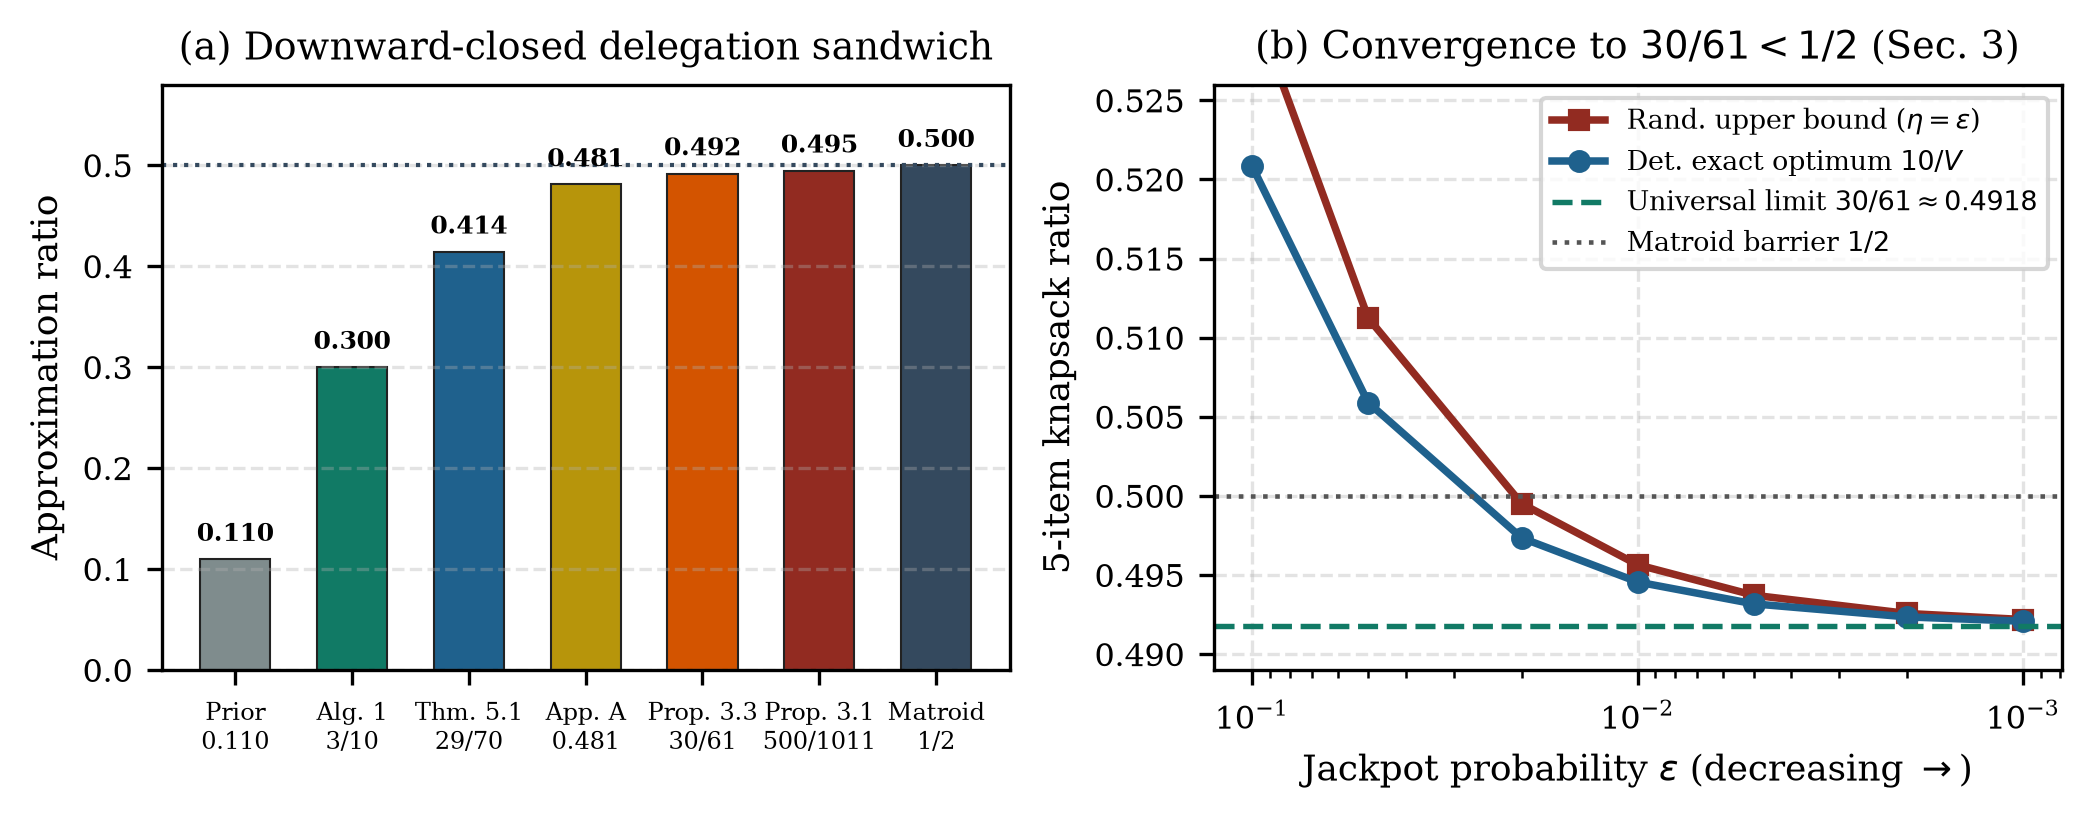
\includegraphics[width=\columnwidth]{figures/fig1_delegation_sandwich.png}
  \caption{(a)~Universal downward-closed delegation approximation sandwich from $0.1098$ through $3/10$ and $29/70$ to the sub-$1/2$ upper bounds ($0.48105$, $30/61$, $500/1011$). (b)~Exact 5-item knapsack deterministic and randomized ratios converging strictly below $1/2$ toward $30/61 \approx 0.4918$ as $\varepsilon \downarrow 0$.}
  \label{fig:sandwich}
\end{figure}

\paragraph{1. Knapsack Separation \& Degree-7 Bernstein Positivity (Figs.~\ref{fig:sandwich}--\ref{fig:bernstein}).}
Figure~\ref{fig:sandwich} displays the complete approximation sandwich~\eqref{eq:sandwich} and tracks the 5-item knapsack deterministic ($10/V$) and randomized ($\eta=\varepsilon$) upper bounds crossing strictly below $1/2$ at $\varepsilon \le 1/50$ and converging monotonically to $30/61 \approx 0.491803$ (reaching $5000/10161 \approx 0.492078$ at $\varepsilon=1/1000$). Figure~\ref{fig:bernstein} plots Lemma~4.4's exact degree-7 polynomial $P(b)$ across $[2/13, 2/3]$ (log $y$-axis: $P(b) \ge 2.66 > 1$ everywhere, with $P(1/2)=\frac{141}{32}=4.40625$ and $P(2/3)=\frac{33250}{729}\approx 45.61$) together with all 16 strictly positive exact rational Bernstein basis coefficients on $[2/13, 2/5]$ ($\min\beta_k = 447966/78125 \approx 5.733965$) and $[2/5, 2/3]$ ($\min\beta_k = 6518/118125 \approx 0.055179$); on the narrower subintervals $[1/4,1/2]$ and $[1/2,2/3]$ in Table~\ref{tab:atlas}, the Bernstein lower bounds tighten to $\frac{129}{128}\approx 1.0078$ and $\frac{141}{32}=4.40625$, respectively, remaining strictly below $P(b)$ throughout.

\begin{figure}[t]
  \centering
  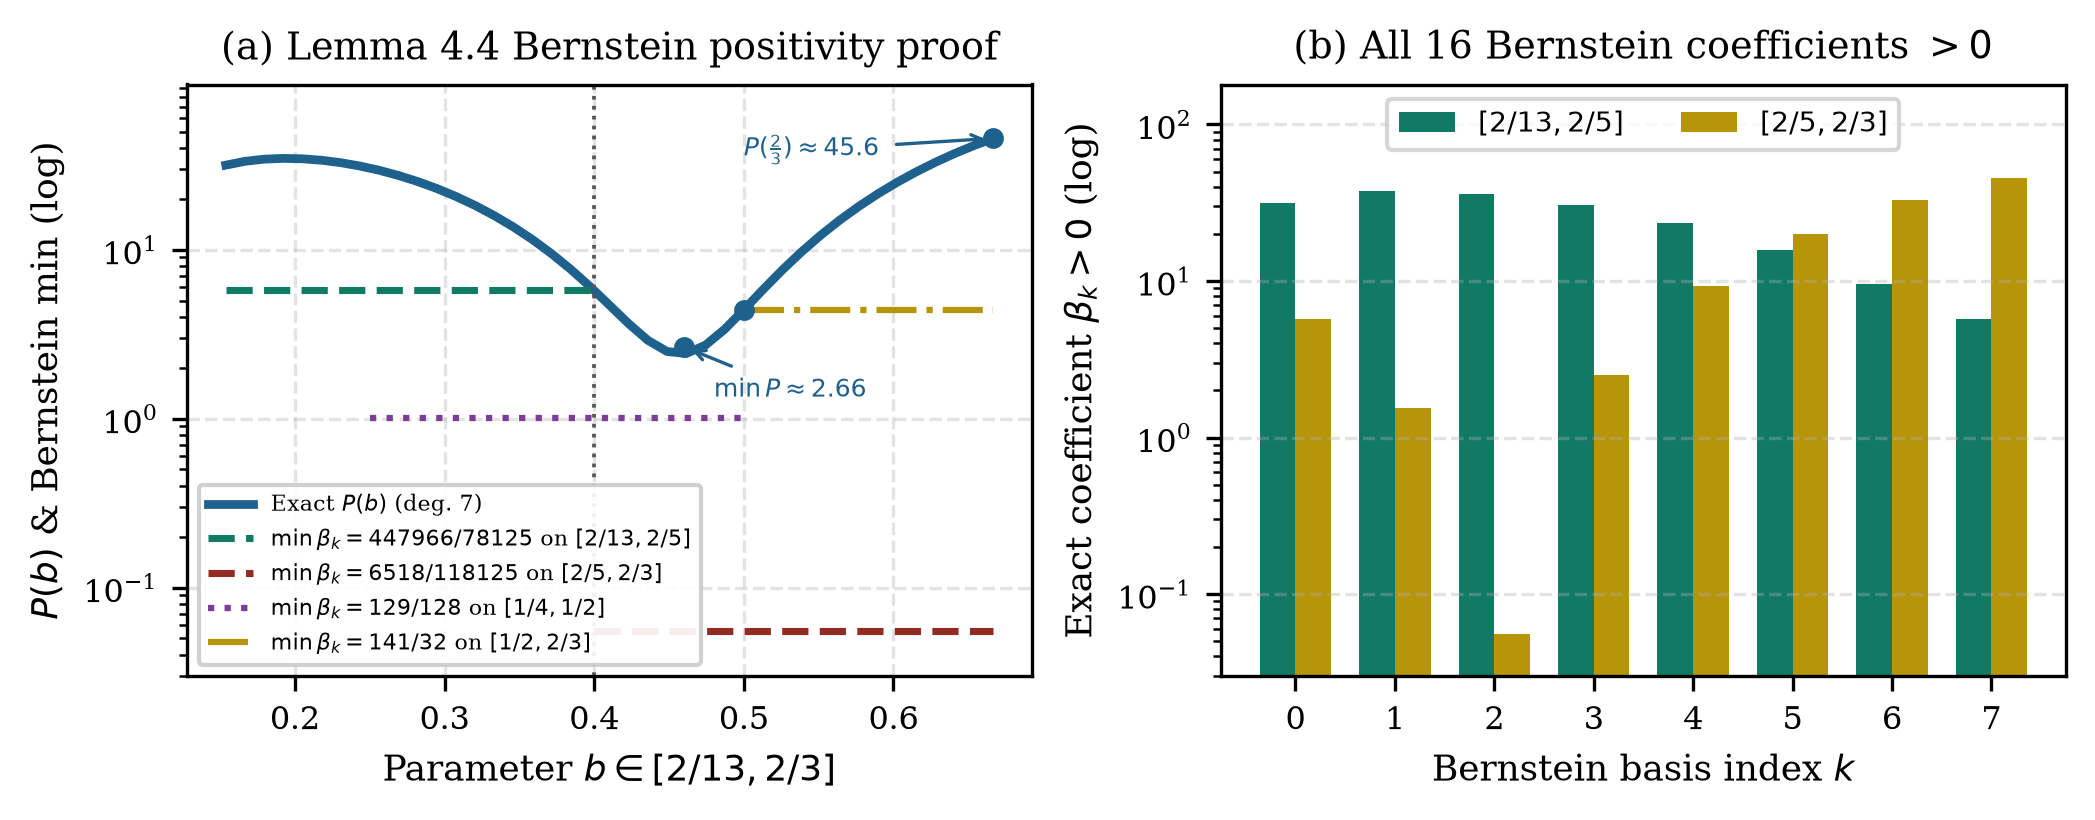
\includegraphics[width=\columnwidth]{figures/fig2_bernstein_positivity.png}
  \caption{(a)~Exact degree-7 polynomial $P(b)$ on $[2/13, 2/3]$ bounded strictly away from zero by its exact rational Bernstein floors on $[2/13,2/5]$ and $[2/5,2/3]$. (b)~All 16 exact rational Bernstein coefficients $\beta_k > 0$ across both subintervals.}
  \label{fig:bernstein}
\end{figure}

\paragraph{2. 16-Certificate Atlas \& 60/60 Red-Team Audit (Table~\ref{tab:atlas}, Fig.~\ref{fig:atlas}).}
All 16 canonical certificates replay in $0.254$--$2.272\,\mathrm{ms}$ with zero floats. On every non-matroid finite test family, Algorithm~2's capped menus (\texttt{threshold}, \texttt{seeds\_upper}, \texttt{seeds\_reserve}) strictly improve over Algorithm~1's single threshold ($67/99 \to 13/18$ on 4-item knapsack, $193/263 \to 201/263$ on $P_4$ independent sets, $43/68 \to 49/68$ on the safe-singleton family) and match the exact deterministic optimum $500/1011$ on Section~3's 5-item knapsack, exceeding $29/70$ on all four instances. In \texttt{tests/test\_suite.py}, 60 live adversarial forgery attacks (16 AST/schema/Unicode-digit/depth-DoS + 11 per mode) plus 2 raw JSON IEEE-754/\texttt{NaN} file checks achieve \textbf{60/60 (100\%)} red-team rejection (63/63 \texttt{pytest} checks passing).

\begin{figure}[t]
  \centering
  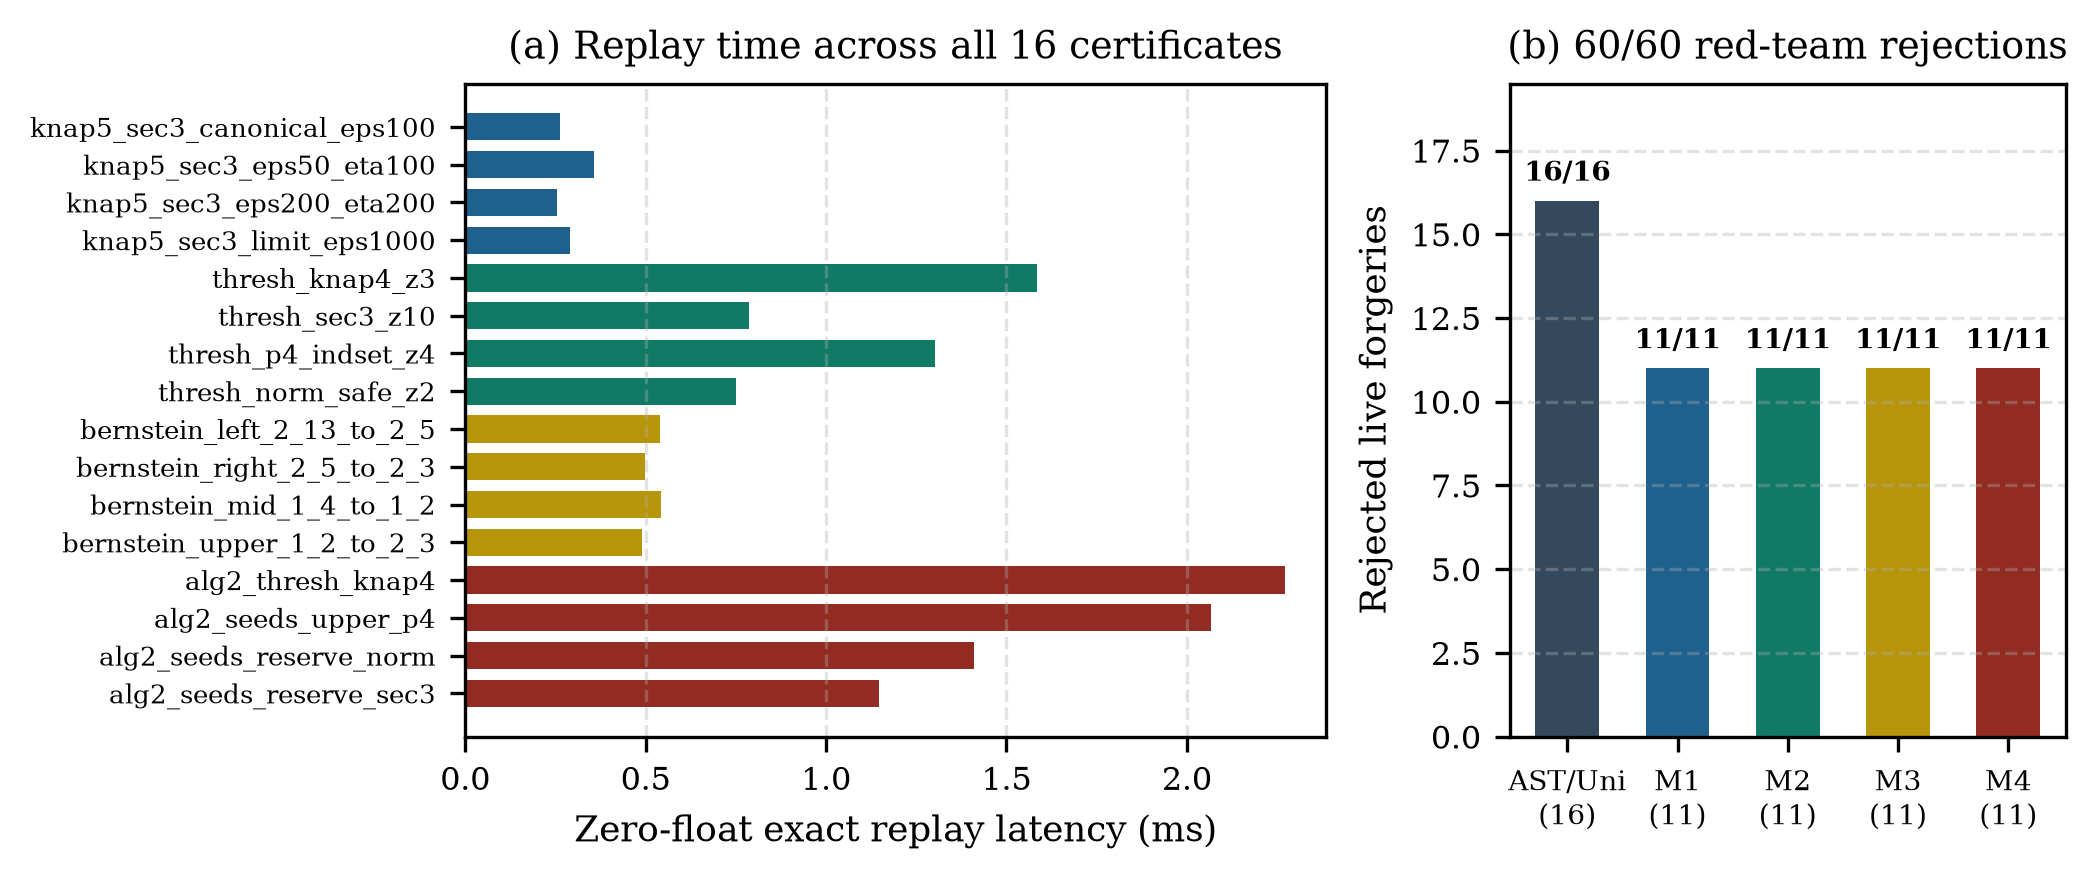
\includegraphics[width=\columnwidth]{figures/fig3_atlas_and_redteam.png}
  \caption{(a)~Zero-float exact replay latency across all 16 canonical \texttt{DELEG-DC-CERT-1.0} certificates ($0.254$--$2.272\,\mathrm{ms}$). (b)~60/60 live adversarial forgery rejections across global AST/Unicode and Modes~1--4.}
  \label{fig:atlas}
\end{figure}

\begin{table}[t]
\centering
\caption{Summary of all 16 exact-$\QQ$ \texttt{DELEG-DC-CERT-1.0} certificates (zero IEEE-754 arithmetic; 20-run mean replay latency in ms).}
\label{tab:atlas}
\resizebox{\columnwidth}{!}{%
\begin{tabular}{@{}lllr@{}}
\toprule
Certificate Stem & Mode & Exact Certified Witness & ms \\
\midrule
\texttt{knap5\_sec3\_canonical\_eps100} & M1 & $V{=}\frac{1011}{50}$, det $\frac{500}{1011}$, rand $\frac{5011}{10110}$ & 0.262 \\
\texttt{knap5\_sec3\_eps50\_eta100} & M1 & $V{=}\frac{1508}{75}$, det $\frac{375}{754}$, rand $\frac{22549}{45240}$ & 0.356 \\
\texttt{knap5\_sec3\_eps200\_eta200} & M1 & $V{=}\frac{6083}{300}$, det $\frac{3000}{6083}$, rand $\frac{2281}{4620}$ & 0.254 \\
\texttt{knap5\_sec3\_limit\_eps1000} & M1 & $V{=}\frac{10161}{500}$, det $\frac{5000}{10161}$, rand $\frac{500111}{1016100}$ & 0.292 \\
\texttt{thresh\_knap4\_z3} & M2 & $V{=}\frac{33}{8}$, ratio $\frac{67}{99}$, $\mathrm{Var}{=}\frac{135}{256}$ & 1.584 \\
\texttt{thresh\_sec3\_z10} & M2 & $V{=}\frac{1011}{50}$, $B{=}10$, ratio $\frac{500}{1011}$ & 0.786 \\
\texttt{thresh\_p4\_indset\_z4} & M2 & $V{=}\frac{263}{48}$, ratio $\frac{193}{263}$, $\mathrm{Var}{=}\frac{983}{576}$ & 1.302 \\
\texttt{thresh\_norm\_safe\_z2} & M2 & $V{=}\frac{17}{6}$, ratio $\frac{43}{68}$, $\mathrm{Var}{=}\frac{311}{576}$ & 0.751 \\
\texttt{bernstein\_left\_2\_13\_to\_2\_5} & M3 & $[\frac{2}{13},\frac{2}{5}]$, $\min\beta_k{=}\frac{447966}{78125}$ & 0.539 \\
\texttt{bernstein\_right\_2\_5\_to\_2\_3} & M3 & $[\frac{2}{5},\frac{2}{3}]$, $\min\beta_k{=}\frac{6518}{118125}$ & 0.498 \\
\texttt{bernstein\_mid\_1\_4\_to\_1\_2} & M3 & $[\frac{1}{4},\frac{1}{2}]$, $\min\beta_k{=}\frac{129}{128}$ & 0.543 \\
\texttt{bernstein\_upper\_1\_2\_to\_2\_3} & M3 & $[\frac{1}{2},\frac{2}{3}]$, $\min\beta_k{=}\frac{141}{32}$ & 0.490 \\
\texttt{alg2\_thresh\_knap4} & M4 & threshold, ratio $\frac{13}{18} > \frac{29}{70}$, 28 seeds & 2.272 \\
\texttt{alg2\_seeds\_upper\_p4} & M4 & seeds\_upper, ratio $\frac{201}{263} > \frac{29}{70}$, 28 seeds & 2.068 \\
\texttt{alg2\_seeds\_reserve\_norm} & M4 & seeds\_reserve, ratio $\frac{49}{68} > \frac{29}{70}$, 14 seeds & 1.410 \\
\texttt{alg2\_seeds\_reserve\_sec3} & M4 & seeds\_reserve, ratio $\frac{500}{1011} > \frac{29}{70}$, 6 seeds & 1.148 \\
\bottomrule
\end{tabular}}
\end{table}

\section{Conclusion}\label{sec:conc}
We delivered a self-contained, zero-floating-point verification suite for Abdi, Banihashem, Hajiaghayi, and Mittal's downward-closed delegation bounds~\cite{abdi2026delegation}, pairing 18 zero-\texttt{sorry}, zero-\texttt{Classical.choice} Lean~4.35.0 theorems with the exact-$\QQ$ auditor \texttt{DELEG-DC-CERT-1.0}, 16 canonical certificates, and 60/60 live adversarial forgery rejections.

\bibliographystyle{plain}
\bibliography{references}
\end{document}
